\documentclass[11pt]{article}

\usepackage{graphicx}
\usepackage{amsmath}
\usepackage[margin=0.8in]{geometry}
\usepackage{float}
\usepackage{caption}
\usepackage{subcaption}

\usepackage{listings}
\usepackage{xcolor}
\usepackage{color}

\definecolor{codegreen}{rgb}{0,0.6,0}
\definecolor{codegray}{rgb}{0.5,0.5,0.5}
\definecolor{codepurple}{rgb}{0.58,0,0.82}
\definecolor{backcolour}{rgb}{0.95,0.95,0.92}

\lstdefinestyle{mystyle}{
	backgroundcolor=\color{backcolour},   
	commentstyle=\color{codegreen},
	keywordstyle=\color{magenta},
	numberstyle=\tiny\color{codegray},
	stringstyle=\color{codepurple},
	basicstyle=\ttfamily\footnotesize,
	breakatwhitespace=false,         
	breaklines=true,                 
	captionpos=b,                    
	keepspaces=true,                 
	numbers=left,                    
	numbersep=5pt,                  
	showspaces=false,                
	showstringspaces=false,
	showtabs=false,                  
	tabsize=2
}

\usepackage{tikz}
\usetikzlibrary{shapes.geometric, arrows}
\tikzstyle{startstop} = [rectangle, rounded corners, minimum width=3cm, minimum height=1cm,text centered, draw=black, fill=red!30]
\tikzstyle{ISR} = [rectangle, rounded corners, minimum width=3cm, minimum height=1cm,text centered, draw=black, fill=green!30]
\tikzstyle{io} = [trapezium, trapezium left angle=70, trapezium right angle=110, minimum width=1cm, minimum height=1cm, text centered, draw=black, fill=blue!30]
\tikzstyle{process} = [rectangle, minimum width=3cm, minimum height=1cm, text centered, draw=black, fill=orange!30]
\tikzstyle{arrow} = [thick,->,>=stealth]



\title{\textbf{MECH 423 Final Project \\
		Bed Occupancy Alarm Clock}}
\author{Dana Deutsch \\
		deutschdana@gmail.com}
\date{November 28th 2020}
\begin{document}
\maketitle
\subsection*{Abstract}
Many people struggle to get out of bed in the morning. 
Whether its because they fall back asleep after turning off their alarms or because they lack motivation to get up it doesn't matter.
This products goal to get get the user out of bed using an alarm system that senses if the user is in bed.
Since nowadays people use their phones for everything, including for alarm clock, the product will be best used if integrated into a phone app with a wireless link to the bed occupancy sensor. 
Unfortunately this is outside the project course timeline, so his product only interfaces with the phone using a sound sensor for the phone alarm.
This external phone alarm sound is detected in order and begins a MSP430 controlled repetitive alarm system that would keep intermittently ringing regardless of how many times you press the off button unless you leave the bed.
Further more it will keep monitoring the bed occupancy for an hour after you leave the bed to ensure you  don't return.\\
\\
The design uses two 50kg load cells positioned under a leg of the bed to sense the bed occupancy.
The voltage signal is amplified using the HX711 amplifier and ADC that tuns it into a digital value that is collected by the MSP430 by bit banging.
The MSP430 tracks two other inputs that are used for creating the alarm system: the snooze button and the sound sensor.
It also uses a piezo buzzer to output the alarm sound and its own internal timers and ISR to control them all. 
The MSP430 controls the system but it also sends data values via serial to a laptop for more data analysis as a way to simulate the benefits of a phone data link for the sensor.
The window form program can record the values collected, calculate how long the user has been in bed, how long the user slept before being woken up, and how long it took the user to wake up.
This project is a functional prototype for a better integrated bed occupancy sensor that can be used for alarm clock systems as well as other functionality like home automation.    

\newpage
\tableofcontents
\newpage

\section{Objectives}
The goal of this project is to create an alarm clock system for people who have a hard time waking up and getting out of bed.
Many people simply turn off their alarms and fall back asleep or just lack the motivation to get up.
They must then set multiple alarms to remind themselves to get up.
This is a temporary solution since you can still turn off all the alarm and stay in bed.
My objective of my system is to eliminate the possibility of remaining in bed by taking away the power to fully "turn off" the alarm while keeping a short "snooze" functionality people can enjoy. 
A consistent alarm that rings while in bed is not beneficial to waking up as it gets annoying fast and stop people from using the device because they are forced to get out of bed right away.  
Since most people don't use a physical alarm clocks and instead use their phones, this projects goal is to also interfaces with the phone people already use in order to add functionality to it instead of removing an already fully perfect functional system.\\
\\
Creating a phone application interface is the preferred solution for this but its outside the scope of this project as it adds a lot complexity. 
Instead this project uses the phone alarm sound as an input point for a bed detecting alarm system which operates separate from the phone on the MSP430.
After the original alarm, the device will periodically ring after the user "snoozes" until the user leaves the bed and doesn't return to bed for a set amount of time.
This way the main alarm can be set on the phone which users already have set up since it has a better interface and more alarm features, but the rest of the system alarm control is run on the a microcontroller. 
The device will sense when the phone alarm goes off in order to begin its functions instead of having its own internal real time clock and alarm setting capacity.
I do want to simulate the possibilities of sending data to a phone app because I believe its an integral part of how this product can be used in real production not DIY usage. 
So I created a serial connection with a PC that displayed the sleep cycle data visually and shows one of the many functionalities this data can be converted into with a phone app.
One of those functionality if a sleep cycle tracker of how long you sleep or spend in bed which I show,but another is connecting to other wireless devices to automate the coffee machine when you wake up.
The future possibilities is endless.\\
\\
\section{Rationale}
I want to make this device since it solves a problem I face daily along with many other people.
Instead of setting up 5 different alarms which are close together and spread out to make sure I get up, I can use this device.
I sometimes ignore my alarms and just decide to keep sleeping so this way I will be forced to get up and hopefully fix my sleeping scheduled.
This product isn't available on the market right so its only achievable by making it myself.
I hope this project will provide a concept functionality prototype for a possible market device that uses this method or a better phone app interface. 
As well many home automation can be made using the bed occupancy detection function like starting the coffee maker when you leave the bed and opening the blinds and more.
In reality this produce can be created as a fully functional phone application with a Bluetooth connection to the load sensor which would allow for way more features.
I want to only simulate this connection with serial to just show how sensing bed values can provide useful data.
This project is quite different then other labs and project because I actually apply the material into something useful and not predefined labs.
This is particularly seen from load sensors which we learn about it MECH 420 but it also uses the rest of the material from MECH 423. 

\section{Functionality Summery}
The hardware components on the system include the microcontroller (MCU), a input bed sensor for the bed, input audio sensor for detecting the phone alarm, output buzzer to create its own alarm sounds, and laptop for the showing the data-steam functionality. 
The main controller is the MCU for every functionality.
The MCU is used to to control the logic for when the buzzer goes off which are based on port interrupts and force sensor inputs. 
The timers are used for waiting between states and well as creating sound with the peizo buzzer.
The MCU code reads the output of the force and sound sensor to detect if the user is in bed and if the phone has rung based on calibration values.
The MCU sends an output signal to play an alternating frequency buzzer for the alarm sounds and a data packet to the laptop. 
I created a few requirements for the functions ordered by importance.
They were also developed in this order and therefore combined in this order after the completion of each function.
The functional requirements are found in Table \ref{tab:FR}.\\
\\
The key feature of the functionality is the bed occupancy detection created by load cells and the control code.
I list below a few requirements I had for the system functions needs to meet.
\begin{itemize}
	\item The alarm code cannot be tricked to stop the loop without waiting for an hour past the alarm
	\item The detection of the user must be integrated without compromising the bed comfort or permanently changing the bed structure 
	\item The detection should not interfere with any bed sheet changes and be easily removable
	\item Buzzer must be laud enough to wake a person from a light sleep since deep sleep wont be achievable in the "snooze time"
	\item The sound detection shouldn't get accidentally triggered by a person talking while on the bed
\end{itemize} 

\begin{table}[H]
	\centering
	\caption{Functional Requirements for The Wake Up System}
	\begin{tabular}{|l|l|l|}
		\hline
		&\textbf{Functions} &Effort \%\\
		\hline
		1&Bed Occupancy Detection Circuitry and Reader& 45\%\\
		2&MCU Alarm Timer Control Code& 40\%\\
		3&Audio Detection and Output &5\%\\
		4&Data Stream Display &10\%\\
		\hline
	\end{tabular}
	\label{tab:FR}
\end{table}
The MSP430 controlled system includes four inputs and outputs.
The inputs include the load cells, the microphone sensor, and the push button.
While the output is the buzzer. 

\section{Bed Occupancy Detection Circuity and Reader}
In order to detect that the user is in bed, I use load cells that are typically found in bathroom scales. 
These are actually half bridge strain gauged load cells made from riveted sheet metal. 
Figure \ref{fig:loadcellproduct} shows an individual cell.
As seen the sensor is placed on one side on the metal part on the side the experiences tension when loaded.
The cell is one piece of metal with a 'flex' center so we load the metal on the flexing center while mounting only the outer ring of the metal and keeping the part above ground to allow for room to have strain.
In order to use strain gauges, we must connect them in a wheatstone bridge circuit seen in figure \ref{fig:Bridge}. 
In the circuit we sense the voltage across the center of the bridge with a provided input voltage. 
The bridge voltage changes as the strain gauge resistor in the bridge increases with tension. 
The voltage I measured across an empty bridge is around 3mV and this value rises slightly when loaded. 
Since this values are so small we need an amplifier.
I am using the HX711 IC on a breakout board that is meant for load cells and is an amplifier and a 24bit ADC, Figure \ref{fig:loadboard}. 
Figures \ref{fig:HX711} and \ref{fig:hx711blocks} show the sensor block diagram and the board schematic.
The data is read from this chip using an output clock pulse signal and a digital input in a method known as bit banging.  
The chip has three setting for different gains which are selected using the number of clock pulses in each read. 
I am using 25 pulse version which has the largest gain (x128) which allows for the smallest range of voltage detection (0-20mV) which is more than enough for my use case.
Figure \ref{fig:hx711Communication} shows this communication method as seen from the data sheet.
Since I don't need to measure the exact weight of the user for this function, only a change is the overall detected weight, I place the sensors at only one corners. 
This makes the device easier to use, install, and over all more adjustable for other beds.
From testing described in later section I knew the loads at a corner is around ~40kg in magnitude which is sufficient for two load cells at one corner.\\
\\
The final circuit for this functionality is then made up of two load cells forming a whetstone bridge read by the HX711 connected to the MSP430 port 1.0 and 1.1 which are input and output ports respectively.
Figure \ref{fig:fullCircuit} shows the entire circuit diagram which has these load cell connections shown with the HX711 breakout board inputs and outputs.
The figure also shows the inputs and outputs for our other connection to the MSP430.
In order to mount the load cells I needed to raise it above the ground to provide round for the strain and to hold the rivets above the ground.
Since I didn't have access to a 3D printed, I mounted the two load cells across the gap of two piles of sticky notes and duct taped only the outer edge in place.
Then I positioned the leg of the bed to press on both directly.
The set up is seen in figure \ref{fig:mechmount} both in the loaded and unloaded positions.
The function of code for reading and averaging the ADC values, global variables named LoadCellVal and Average respectively, via bit banging is seen in listing \ref{ADCCode} below.    
\\
\begin{figure}[H]
	\centering
	\begin{subfigure}[]{0.4\textwidth}
		\centering
		\includegraphics{loadcellback}
		\caption{Back}
	\end{subfigure}
	\hfill
	\begin{subfigure}[]{0.4\textwidth}
		\centering
		\includegraphics{loadcellfront}
		\caption{Front}
	\end{subfigure}
	\caption{The Load Cells Used}
	\label{fig:loadcellproduct}
\end{figure}
\begin{figure}[H]
	\centering
	\includegraphics[width = 0.4\linewidth]{bridgeConnefiguration}
	\caption{Measuring Across a Wheatstone Bridge}
	\label{fig:Bridge}
\end{figure}
\begin{figure}[H]
	\centering
	\includegraphics[width = 0.4\linewidth]{bridgeConnefiguration}
	\caption{Measuring Across a Wheatstone Bridge}
	\label{fig:loadboard}
\end{figure}
\begin{figure}[H]
	\centering
	\includegraphics[width = 0.7\linewidth]{hx711applicationBlock}
	\caption{Function Block Diagram for the HX711 Chip}
	\label{fig:hx711blocks}
\end{figure}
\begin{figure}[H]
	\centering
	\includegraphics[width = 0.7\linewidth]{HX711}
	\caption{Schematic for the HX711 Load Sensor Board}
	\label{fig:HX711}
\end{figure}
\begin{figure}[H]
	\centering
	\includegraphics[width = 0.8\linewidth]{exampleDatashaeet}
	\caption{Communication for the HX711 Example from Data Sheet}
	\label{fig:hx711Communication}
\end{figure}
\begin{figure}[H]
	\centering
	\begin{subfigure}[]{0.4\textwidth}
		\centering
		\includegraphics{unloadedCells}
		\caption{Back}
	\end{subfigure}
	\hfill
	\begin{subfigure}[]{0.4\textwidth}
		\centering
		\includegraphics{ loadedCells}
		\caption{Front}
	\end{subfigure}
	\caption{The Load Cells Used}
	\label{fig:mechmount}
\end{figure}
\begin{figure}[H]
	\centering
	\includegraphics[width = 0.8\linewidth]{fullscem}
	\caption{Communication for the HX711 Example from Data Sheet}
	\label{fig:fullCircuit}
\end{figure}
\begin{lstlisting}[label=ADCCode,caption=AX711 Reader Functions For Single ACD Value and Average, language = C,frame=single]
	void ReadAverageForce(){
		unsigned char count = 0;
		unsigned char numtoAve = 5;
		LoadCellVal = 0;
		for(count = numtoAve; count>0;count--){
			ReadForce();
			Average +=LoadCellVal
		}
		Average = Average/numtoAve;
	}
	
	void ReadForce(){
		unsigned char counter =0;
		unsigned long ReadVal=0;
		while(P1IN & BIT0){};
		ReadVal =0;
		for(counter = 24 ; counter >0;counter--){
			P1OUT |= BIT1;
			ReadVal = ReadVal<<1;
			P1OUT &= ~BIT1;
			if(P1IN & BIT0){
				ReadVal |= 0x01;
			}
		}
		P1OUT |= BIT1;
		ReadVal = ReadVal ^ 0x800000;
		P1OUT &= ~BIT1;
		LoadCellVal = ReadVal;
	}
\end{lstlisting}

\subsection*{Inputs and Outputs}
The input to this function is the person providing force by laying on the bed.
This translates to the voltage across the bridge and transfered by the HX711 into a digital input for the MSP430.
This input value is read from the HX711 digital output using an output clock signal for the HX711 bit banging. 
As well, we provide the supply voltage VCC from the MCU for the sensor circuit.

\subsection*{Parameters}
The main parameter is the voltage value which is measured across the bridge which translates as to the value we read from the ADC by the HX711.
I chose the largest gain for the HX711 because I knew it always stays below 20mV from testing which is my second parameter. 
The third parameter I chose was the number of load cells to use and at how many legs. 
As I mentioned before and seen in the next section this came from testing the wight of the bed and the user and finding the supported values and adding a safety margin. 
It is also better to not load the cell at its full scale output because they causes more drift and error. 

\subsection*{Testing}
I began my tested with concept testing by taking apart a bathroom scale and placing the load cells under the bed, figure \ref{fig:preliminary}.
From concept testing I devised that placing two sensors under the corner of the bed should be sufficient since each sensor supports up to 50kg. 
The rough measurements I got from my preliminary test was around 32kg appearing at the far most edge of the bed corner with myself laying on the bed.
In this picture I show an empty bed at 17kg.
So my set up can allow for my full mass load to be placed on one leg and still remain below the FSO of the load cell. \\
\\
While building the circuit I tested to make sure my load cells are outputting voltage reading correctly using the Analog Discovery.
Connecting the circuit I measured the bridge voltage to check that Im getting voltage readings in the mV and that pressing on the cells increases was increasing the reading signifying my ADC values will be increasing as desired.
Figure \ref{fig:bridgevoltage} shows this reading which was around 2mV in this image and fluctuated as it was noisy before the low pass filter and amplifier on the hx711 board. 
\\
Once I had the circuit working I tested the reader functions by measuring outputs while in bed at different positions and over a 5hr period to make sure a dont see a huge drift in the value for some reason.
I recorded the empty and occupied bed values to note is measurements change.
I did notice that any repositioning of the load cell will change the values so its important for me to set a passing criteria value that is close to the empty bed value but not too close to have accidental triggers.
I decided to make the final adjustments for passing criteria after the full system is built since I wanted to use a bed leg that is harder to reach and position and therefore the testing for this was done on another leg.
The final passing paramater for the load cell reader code is determained right before conducting a test by measuring an empty bed, adding 0.1million to the value and rounding up to nearest 0.05million.  
The value I used for the chosen bed leg was 8,650,000.
The values I recorded for the empty bed are \textbf{around while the occupied bed varies between.}
 
\begin{figure}[H]
	\centering
	\includegraphics[width = 0.5\linewidth, angle = 270]{preliminarytest}
	\caption{Preliminary Test With Bathroom Scale}
	\label{fig:preliminary}
\end{figure}
\begin{figure}[H]
	\centering
	\includegraphics[width = \linewidth]{emptyBridgeReading}
	\caption{Voltage Reading of Unloaded Bridge Powered with 5V}
	\label{fig:bridgevoltage}
\end{figure}
\newpage

\section{Main MCU Timing Code for Alarms}
\subsection*{Approach and Design}
The MCU is the control behind when the alarms go off based on our hardware inputs. 
The flowchart to the logic behind the alarms are found in figure \ref{fig:flow}.
The premise of the flow of the states it that there are 4 main stages: Waiting for alarm, waiting between buzzers , getting the user up to press snooze while ringing, and checking that the user remains out of bed.   
First we have the waiting for the sound input, which needs to reset some values before waiting for an ISR on Port 1 to initiate by the Push button.
The ISR checks if the user is in bed at the time of the alarm.
If they are then then we move to the next stage of getting them out of bed, but they they arn't, then we move to the stage of ensuring they stay away from the bed.
The reason for this is that sometimes you get up a few minutes before the alarm and can maybe go to the washroom and return to bed later.
We want to ensure that regardless of their location they stay away from the bed for an hour to fully wake up.  
In order to get the user up the buzzer goes off intermittently which forces the user to keep getting up to shut it off which doesn't let them fall back into a real sleep.
We wait for a set amount of second using TB1 and then ring buzzer and wait for an ISR on Port 4.
We repeat this loop checking every time our wait finished wether the buzzer is required based on bed status. 
Finally our last stage is counting up to an hour while the user is out of bed. 
in this stage we check intermittently so the user can still sit down on the bed maybe to scroll on reddit for a min before being reminded to get up.  
I found that an intermittent reminder is more user friendly then a constant check and does a better job to get you up. \\
\\
The code uses 8 states in an infinite loop which relays on the use of a one second timer interrupt, and port interrupts.
The one second timer interrupt is used to count the 'waiting' time between the alarms and counting the second 1hr out of bed check sequence.
The timer is always running so when ever we need to use it we can count the number of interrupts and preform tasks accordingly. 
Its also used to send serial data to the computer and to time between the frequency changes of the buzzer discussed in next sections. 
The code was first written with the buzzer and force sensor as digital input/outputs simulated using the analog discovery before combining their real functions.  
The fully final code is found in appendix \ref{sec:code}.
\\
\begin{figure}[H]
	\centering
	\label{fig:flow}
	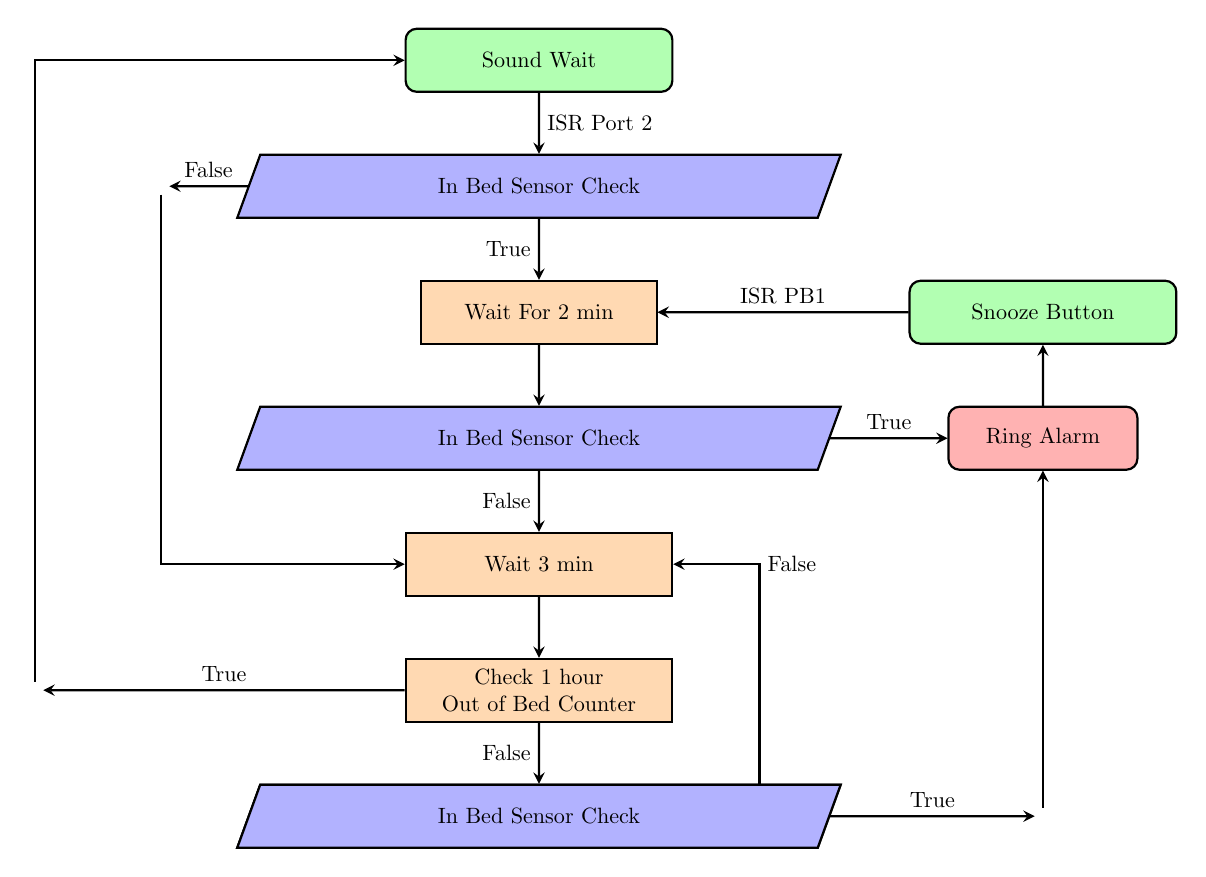
\begin{tikzpicture}[node distance =2cm, thick,scale=0.9, every node/.style={scale=0.8}]
		
		\node (Realtime) [ISR,text width=4cm ] {Sound Wait}; 
		\node (InBed3) [io, below of=Realtime,text width=4cm] {In Bed Sensor Check};	
		\node (Wait1) [process, below of=InBed3,text width=3.5cm] {Wait For 2 min };
		\node (snoozePB) [ISR, right of=Wait1,text width=4cm, xshift = 6cm] {Snooze Button};
		\node (InBed) [io, below of=Wait1,text width=4cm] {In Bed Sensor Check}; 
		\node (Ring1) [startstop, right of =InBed, xshift = 6cm] {Ring Alarm};
		\node (wait2) [process, below of=InBed, text width=4cm] {Wait 3 min};
		\node (counter) [process, below of=wait2, text width=4cm] {Check 1 hour \\Out of Bed Counter};
		\node (InBed2) [io, below of=counter, text width=4cm] {In Bed Sensor Check}; 
		\node (return1) [right of=InBed2, xshift =6cm]{};
		\node (return2) [left of=counter, xshift =-6cm]{};
		\node (return3) [left of=InBed3, xshift =-4cm]{};
		\node (return4) [right of=InBed2, xshift = 1.5cm]{};
		
		
		\draw [arrow] (Realtime) -- node[anchor=west] {ISR Port 2}(InBed3);
		\draw [arrow] (InBed3) -- node[anchor=east] {True}(Wait1);
		\draw [arrow] (InBed3) -- node[anchor=south] {False}(return3);
		\draw [arrow] (return3) |- (wait2);
		\draw [arrow] (Wait1) -- (InBed);
		\draw [arrow] (Ring1) -- (snoozePB);
		\draw [arrow] (snoozePB) -- node[anchor=south]{ISR PB1} (Wait1);
		\draw [arrow] (InBed) -- node[anchor=south] {True} (Ring1);
		\draw [arrow] (InBed) -- node[anchor=east] {False} (wait2);
		\draw [arrow] (wait2) --  (counter);
		\draw [arrow] (counter) -- node[anchor=south] {True} (return2);
		\draw [arrow] (counter) -- node[anchor=east] {False}(InBed2);
		\draw [arrow] (return1) -- (Ring1);	
		\draw [arrow] (InBed2) -- node[anchor=south]{True}(return1);	
		\draw [arrow] (return2) |- (Realtime);
		\draw [arrow] (return4) |- node[anchor=west]{False} (wait2);
		\node (InBed5) [io, below of=counter, text width=4cm] {In Bed Sensor Check}; 
	\end{tikzpicture}
	\caption{Flowchart for the Alarm Actuation Logic}
\end{figure}

\subsection*{Inputs and Outputs}
The main input is the determined output from the bed occupancy detection. 
This will be an ADC read value to determine if the level passed the set calibrated value and the person is in bed. 
The second input is the output from the phone audio sensor which actuates the entire flow chart. 
The third input is a snooze button for the user to temporarily turn off the alarm.
Finally we have the output buzzer to get the user out of bed which will be set with a PWM signal that changes frequencies of different sounds. 
For this function build they were tested using simple IO signals instead of the real sensors.

\subsection*{Parameters}
The software will check and use the following to function and later add the parameters from other sections:
\begin{itemize}
	\item The state of the bed as a digital high or low
	\item The state of the audio volume as a digital high or low 
	\item Count in seconds the timer interrupt needs to pass before snooze alarm needs to start
	\item Count in seconds the timer interrupt needs to pass before secondary check needs to recheck bed status
	\item Count of number of times the secondary timer check loop has gone off to provide enough time for out of bed detection (1hr)
	\item The comparison value for the previous three counting variables 
\end{itemize}


\subsection*{Testing}
Testing was preformed using test cases based on the state machine. 
I pretended to be the user using the simulated inputs and outputs and went through the stages of the flowchart.
I did this over and over again and kept preforming these as the code changed with additional function combination. 

\section{Phone audio detection and audio output}
\subsection*{Approach and Design}
This function encompasses the two sound related traducers I plan to use and the code controlling them.
It also includes connecting them to the previous section of code, so while testing in this function I actually combined all my sensors to my code including the load cell reader passing criteria.
To detect the phone alarm, as long as the phone is placed right on top of the product, I can measure the volume of sounds and only actuate on laud enough sounds using a microphone. 
I found a microphone attached with a audio amplifier board seen in figure \ref{fig:audioboard}.
The schematic of this board is found in figure \ref{fig:audioscem},
The board has a both analog and digital inputs where the analog is the non amplified signal with an reference.
I planned to test both and see which one work best and I found that adjusting the resistor on the board which controls the level at which the digital output changes is sufficient for the application since the microphone on the board was not picking up quite sound only larger ones like the alarm blaring reside it or dropping a large book on my desk. 
I used an ISR to trigger the code when the input signal from the sensor goes high and to MSP430 port.  
To create the output alarm I used a piezo buzzer board which has the switching controller on board so I didn't need an external mosfet and just had to provide a digital PWM signal along with my Vcc.
I change between two different frequencies for the buzzer timer which are swapped every 1sec while we are on via the one second timer interrupt.
The frequencies represent the real sound frequency we hear.  

\begin{figure}
	\centering
	\includegraphics[width = 0.2\linewidth]{soundsensor}
	\caption{The Audio board in Plan}
	\label{fig:audioboard}
\end{figure}
\begin{figure}
	\centering
	\includegraphics[width = 0.8\linewidth]{SoundScem}
	\caption{Microphone Board Schematic}
	\label{fig:audioscem}
\end{figure}

\subsection*{Inputs and Outputs}
The output to the buzzer system is a PWM signal that switches the piezo buzzer to create the sound.
In particular this comes from a timer output from the MSP430 which we change the frequency of. 
As well the input to the microphone is the sound of the phone alarm to the microphone that creates the signal for detection.

\subsection*{Parameters}
The first parameter is the resistance we need to calibrate the sound sensor to provide a digital high signal when the alarm goes off but not in other less laud noises.
This is adjusted with the variable resistor on the board while the phone alarm is on. .
The second value is the frequency which we send to the buzzer to create different frequency sounds.
I chose this frequencies based on two high frequencies humans can hear and just played around to get what I though was an annoying frequency pair.    

\subsection*{Testing}
The test plan for the buzzer is simple, see if the sound is outputted and is heard well enough. 
For the microphone I want to test various phone alarm tones to check it can detect them and detain how close or far away to the microphone I need to be in order to trigger my code. 
 
 
\section{Window Form Display}
\subsection*{Approach and Design}
The goal of the display is to add a data stream from the MSP430 without actually controlling the alarm code. 
This makes the display optional since having a computer beside the bed is sometimes difficult and wasteful keeping it always on and recording data.
The serial connection is therefor a one direction connection where a data packet is send to the PC.
This input packet is described in the input and outputs section below.
The data link doesn't disconnect from the computer as long as the computer is one which is done by changing the power setting and using a sync byte.
The data displayed is the current ADC value along with the current time the user has been in bed for or the last amount of time in bed if the user is out of the bed.
The two main data values we collect from the display is the time it takes the user to wake up and how long they have slept for before the alarm woke them up. 
This allows the user to see their progress and hopefully they will get more sleep and wake up faster while using the device. 
Figure \ref{fig:UI} shows the displayed output for data collection.
As well the data can be outputted as a csv files which is useful in testing. 
 \begin{figure}
 	\centering
 	\includegraphics[width = 0.8\linewidth]{UI}
 	\caption{User Data Display }
 	\label{fig:UI}
 \end{figure} 

\subsection*{Inputs and Outputs}
The input of this function is a serial packet sent by the code in the one second timer. 
The packet is described in Table \ref{tab:packet}.
The data bytes are the 24bit ADC value and the command byte gives information on the state of the alarm cycle. 
I did notice some bytes get lost when the computer is just unlocked so the Sync byte is very important.
This serial connection isn't a perfect solution its unreliable and require continuous connection via a cable. 
Maybe in the future I will connect it to a wifi or bluetooth module instead.
The output is the display user interface and a CSV output recording of the ADC values. 
\begin{table}[H]
	\centering
	\caption{Approximate Contour Errors relative to Feed Rate}
	\label{tab:packet}
	\begin{tabular}{|l|l|l|l|l|}
		\hline
		Sync  & Data 1 & Data 2 & Data 3 &Command \\
		\hline
		255 &  \multicolumn{3}{c|}{ADC 2 Compliment Value}  & 0 - nothing  \\
		 &  \multicolumn{3}{c|}{}  & 	1 - alarm sounded \\
		 &  \multicolumn{3}{c|}{}  &	2 - cycle ended \\
		\hline	
	\end{tabular}
\end{table}
\subsection*{Parameters}
the first parameter I chose was how often to send the data packet.
Since the program operates in minutes and hours, no one really measures how long they sleep in seconds, I determined that it doesn't need to be too precise and so that using DateTime objects is better then the serial sending rate.    
I decided to send the pack once a second in the same timer interrupt that is always on because it is just good enough for testing functionality in the range of tens of seconds while still working well in the range of minutes. 
Sending the packet too fast will just cause too many useless data points.
Below are a list of parameters used in the C\# program. 
They are used to determine the time values displayed on the interface. 
\begin{itemeize}
	\item DateTime at start of program
	\item DateTime at the time the user entered the bed detected by ADC value changing from the data stream
	\item DateTime when the alarm rung detected via the the steam command byte
	\item DateTime when the user left the bed detected by ADC value changing from the data stream
	\item Current ADC value 
	\item DateTime when the alarm cycle has finished
	\item Current time
\end{itemeize}

\subsection*{Testing}


\section{System Evaluation}

\section{Reflection}

\end{document}